\documentclass[tikz,border=5mm]{standalone}
\usepackage{amsmath}
\usetikzlibrary{arrows.meta, bending}

\begin{document}
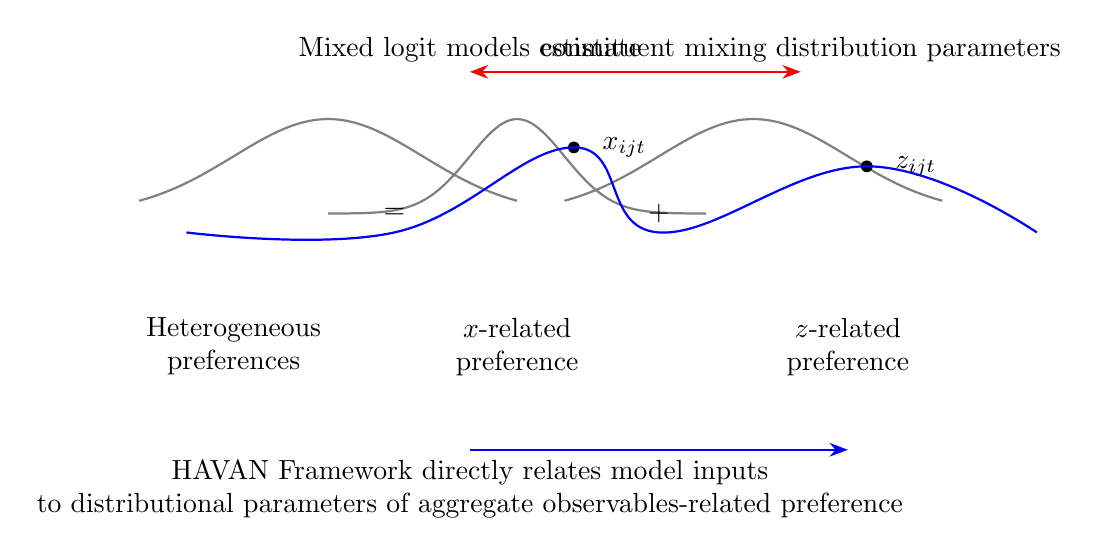
\begin{tikzpicture}[scale=1.2]

% Define styles for clarity
\tikzset{
    curve/.style={thick, domain=-2:2, samples=100},
    arrow/.style={->, >=Stealth, thick},
    dot/.style={circle, fill=black, inner sep=1.5pt},
}

% Left side: Heterogeneous preferences
\draw[curve, gray] plot (\x,{exp(-0.5*\x*\x)});
\node[below, text width=3cm, align=center] at (-1,-1) {Heterogeneous \\ preferences};

% Middle: x-related preference
\draw[curve, gray] plot ({2+\x},{exp(-2*(\x*\x))});
\node[below, text width=2cm, align=center] at (2,-1) {$x$-related \\ preference};
\node[dot] at (2.6, 0.7) {};
\node[right] at (2.8, 0.7) {$x_{ijt}$};

% Right: z-related preference
\draw[curve, gray] plot ({4.5+\x},{exp(-0.5*(\x*\x))});
\node[below, text width=2cm, align=center] at (5.5,-1) {$z$-related \\ preference};
\node[dot] at (5.7, 0.5) {};
\node[right] at (5.9, 0.5) {$z_{ijt}$};

% Equal sign
\node at (0.7,0) {$=$};

% Plus sign
\node at (3.5,0) {$+$};

% Curved blue line connecting the distributions
\draw[blue, thick] plot[smooth, tension=0.7] coordinates {(-1.5,-0.2) (0.7,-0.2) (2.6,0.7) (3.5, -0.2) (5.7,0.5) (7.5,-0.2)};

% Red curved arrow at the top
\draw[red, thick, <->, >=Stealth, bend left=45] 
    (1.5,1.5) node[above, black] {Mixed logit models estimate} 
    -- (5,1.5) node[above, black] {constituent mixing distribution parameters};

% Blue curved arrow at the bottom
\draw[blue, thick, ->, >=Stealth, bend right=45] 
    (1.5,-2.5) node[below, black, align=center] {HAVAN Framework directly relates model inputs \\ to distributional parameters of aggregate observables-related preference} 
    -- (5.5,-2.5);

\end{tikzpicture}
\end{document}